\section{System-Theoretic Process Analysis - STPA}
\label{sec:stpa}

\subsection{Metode}

\begin{figure}[H]
    \centering
        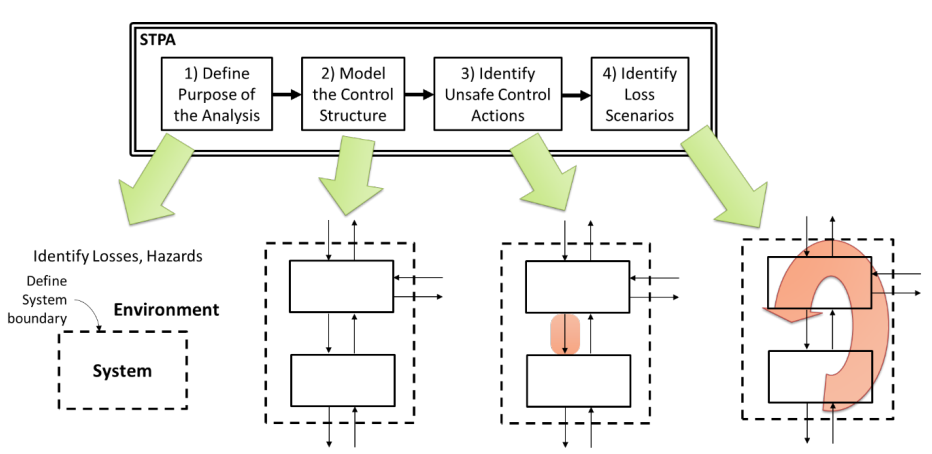
\includegraphics[width=\textwidth]{figures/STPÅ/stpamethod.PNG}\\
        \caption{Oversikt over stegene i STPA-metoden.}
\end{figure}


\subsubsection{Steg 1: Definer formålet med analysen}

I steg 1 skal tap, potensielle hazards og systembegrensninger (constraints) defineres. 
For å definere systemnivå hazards må vi først definere systemet og systemgrensene. Hva skal inkluderes i systemet og ikke?

\begin{itemize}
    \item[\textbf{1}]: Identifiser tap, dvs noe vi potensielt kan miste dersom systemet ikke oppfører seg som ønsket, f. eks. penger, livskvalitet, kundefornøydhet. List dem som "L-1: Tap av liv eller skade på folk, L-2: ...".
    \item[\textbf{2}]: Identifiser system-nivå farekilder (hazards). ISTPA defineres hazard som en systemtilstand som, sammen med et sett av worst-case miljøbetingelser, leder til et tap. List dem, sammen med tapene de potensielt kan føre til "H-1: Båten kommer for nærme andre båter [L-1], H2: ..."
    \item[\textbf{3}]: Definere systemnivå begrenssninger (constraints): Tilstander eller oppførsel som må være oppfylt for å unngå farekilder (hazards), og til slutt forebygge tap. List dem sammen med hazardene de skal unngå, som "SC-1: Båt må opprettholde minimum distanse på 10 m fra andre båter [H-1]".
    \item[\textbf{4}]: Valgfritt: raffinere systemnivå farekilder (hazards): Del hazardsene inn i sub-hazards om ønskelig.
\end{itemize}

Musefelle-eksempel på to runder med dette:

\textbf{Definere systemgrenser}:

\begin{itemize}
    \item \textbf{Objekter}: Musefella, eier av området, åte
    \item \textbf{Aktører}: Musefella og eier av område
    \item \textbf{Mekanismer/funksjoner/Mål:} Drepe mus, Legge på åte, «lade» musefella
    \item \textbf{Miljø} (utenfor vårt system, men som kan påvirke, eller blir påvirket av vårt system):
    \begin{itemize}
        \item Objekter: Hytte, mus, andre dyr, …
        \item Aktører: Mus, andre dyr og fugler (f.eks. rev, ekorn, røyskatt, mink, kråke, ugle), naboen, regelverk, barna, …
        \item Mekanismer: Tiltrukket av åte, Spise åte, Hindre musefellas funksjon, Spise mus, Flytte musefelle, Utløse musefelle,…
    \end{itemize}

\end{itemize}

 Det å ha et bevist forhold til CESM i denne fasen er verdifullt da vi
allerede har indikasjoner på at ikke alt trenger å fungere slik vi hadde tenkt.

\textbf{Runde 1}:

\begin{itemize}
    \item Tap: Tap av livskvalitet 
    \item Hazard: Sykdom [L-1]
    \item Safety-constraint: Unngå smitte
\end{itemize}

\textbf{Runde 2}:

Refined hazard: Smitte fra mus [L-1]. Mer på musefelle-nivå:
\begin{itemize}
    
    \item H-1: Musefelle dreper ikke mus [L-1]
    \item SC-1: Musefelle må lukke seg for å drepe den [H-1]

\end{itemize}

\subsubsection{Steg 2 - Modellere hierarkisk kontrolldiagram}

Et hierarkisk kontrolldiagram er en systemmodell som består av kontroll-tilbakekoblinger. En effektiv kontrollstruktur vil pålegge begrensninger (constraints) på hele systemets oppførsel.

Eksempel:

\begin{figure}[H]
    \centering
        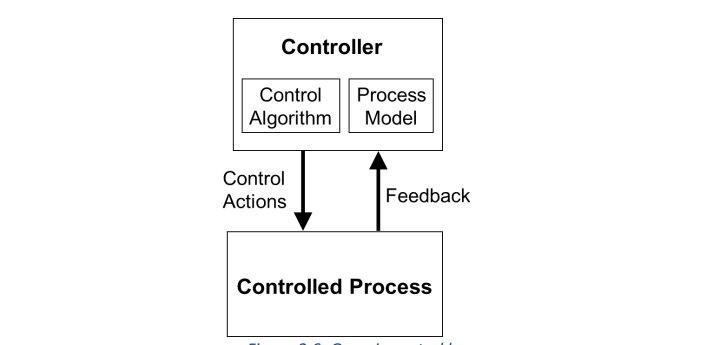
\includegraphics[width=\textwidth]{figures/STPÅ/hier.PNG}\\
        \caption{Generisk kontroll-tilbakekobling.}
\end{figure}

Eksempel fra musefelle-case:

\begin{figure}[H]
    \centering
        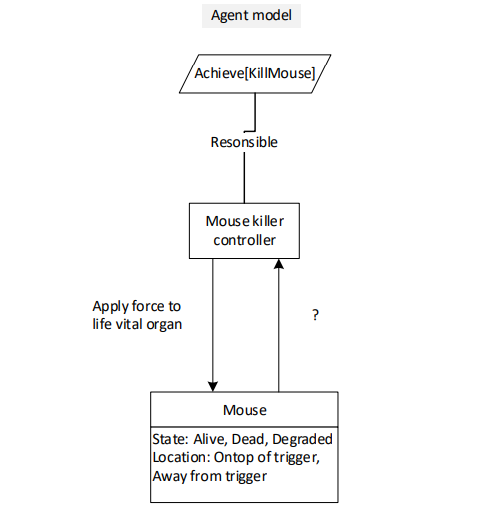
\includegraphics[width=0.5\textwidth]{figures/STPÅ/mus_kontroll.PNG}\\
        \caption{Musefelle-kontrollstruktur.}
\end{figure}

\textbf{Merk}: Kontrollstrukturene kan se veldig annerledes ut, avhengig av hva de skal sette søkelys på. 

\begin{figure}[H]
    \centering
        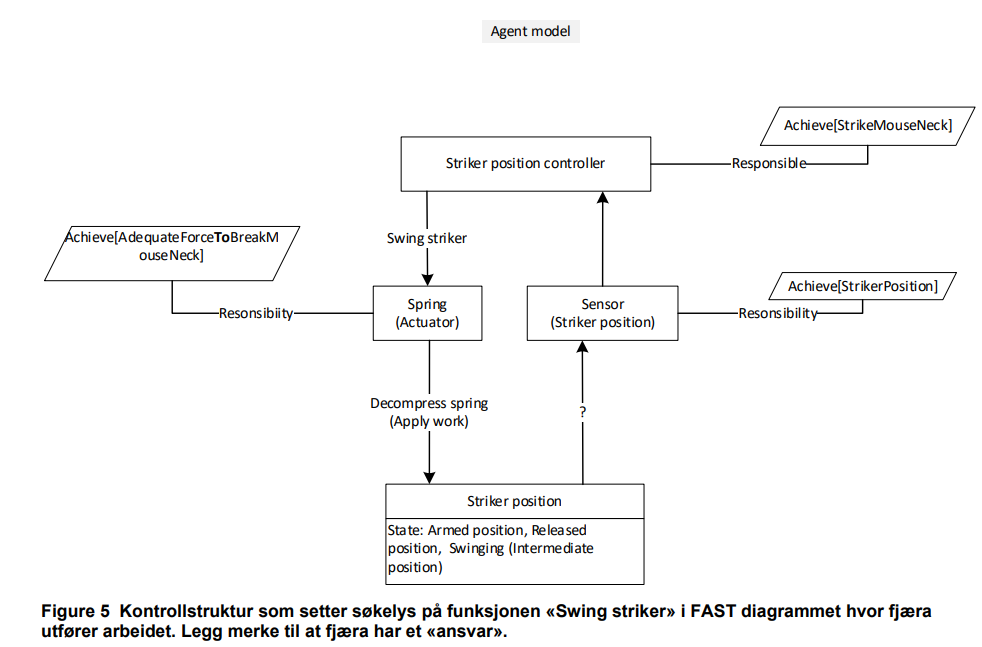
\includegraphics[width=0.5\textwidth]{figures/STPÅ/spring.PNG}\\
        
\end{figure}

\subsubsection{Steg 3 - Identifiser usikre kontrollhandlinger (unsafe control actions)}

Når kontrolldiagrammet er laget, kan vi identifisere usikre kontrollhandlinger. Disse skal listes opp i en tabell og knyttes mod hazardsene som ble definert i steg 1. Eksempel fra STPA-håndbok:


\begin{figure}[H]
    \centering
        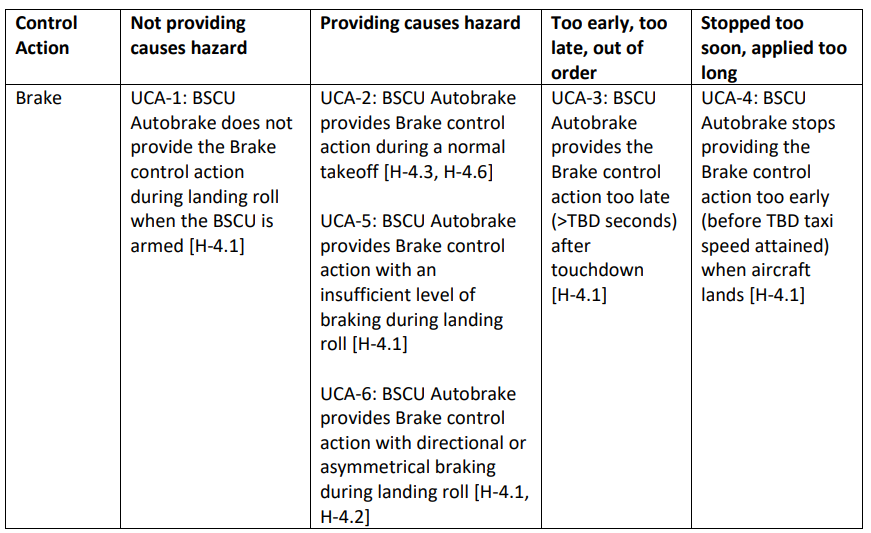
\includegraphics[width=0.8\textwidth]{figures/STPÅ/eks_brake.PNG}\\
        \caption{Eksempel på hvordan man definerer UCAs.}
\end{figure}

Musefelle-eksempel:

\begin{figure}[H]
    \centering
        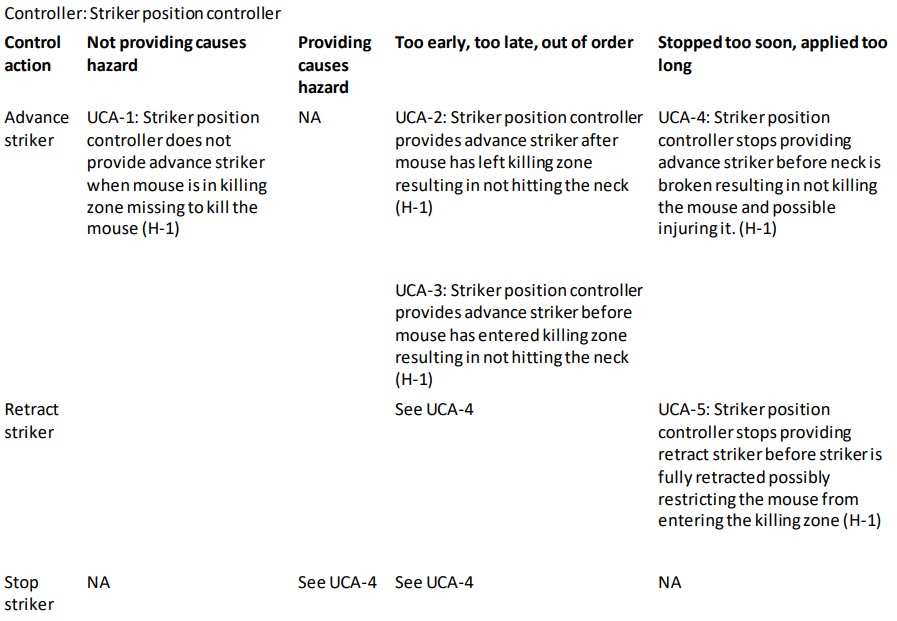
\includegraphics[width=\textwidth]{figures/STPÅ/striker.PNG}\\
        \caption{UCAs i musefelle-eksempel.}
\end{figure}


\textbf{Identifisere safety constraints fra UCAs:}
Når UCA-ene er blitt definert, kan vi oversette disse til begrensninger for systemet som må oppfylles for å forhindre nettopp disse UCA-ene. 

Eksempel fra STPA-håndbok:


\begin{figure}[H]
    \centering
        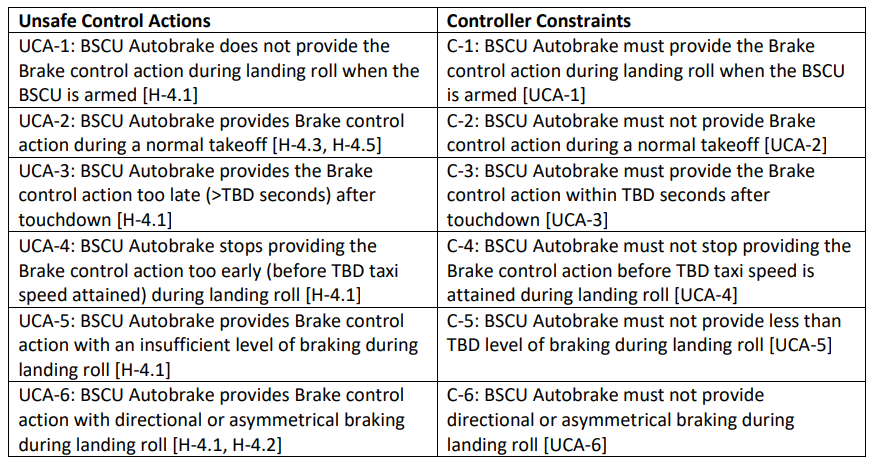
\includegraphics[width=0.9\textwidth]{figures/STPÅ/sc_eks.PNG}\\
        \caption{Eksempel på hvordan man definerer SCs fra UCAs.}
\end{figure}

Eksempel fra musefelle-analyse:

\begin{figure}[H]
    \centering
        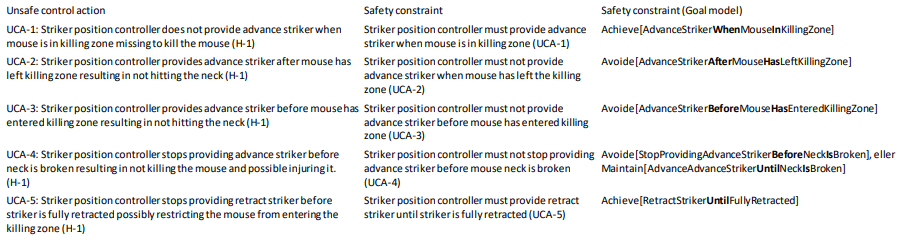
\includegraphics[width=\textwidth]{figures/STPÅ/sc_mus.PNG}\\
        \caption{Eksempel på hvordan man definerer SCs fra UCAs fra musefelle-eksempel.}
\end{figure}

\subsubsection{Steg 4 - identifisere taps-scenarioer}

I steg 4 skal man finne scenarioer hvor UCA-ene kan oppstå, ved å gå rundt kontrollstrukturen for å finne mulige årsaker.

Det gjøres slik, illustrert i håndboken:

\begin{figure}[H]
    \centering
        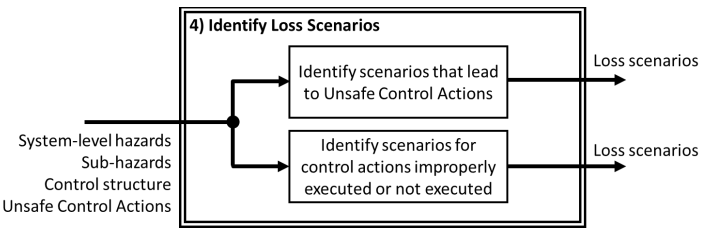
\includegraphics[width=0.9\textwidth]{figures/STPÅ/step4.PNG}\\
        \caption{Steg 4 - definere tapsscenarioer.}
\end{figure}

Eksempel fra musefelle-analyse:

\begin{figure}[H]
    \centering
        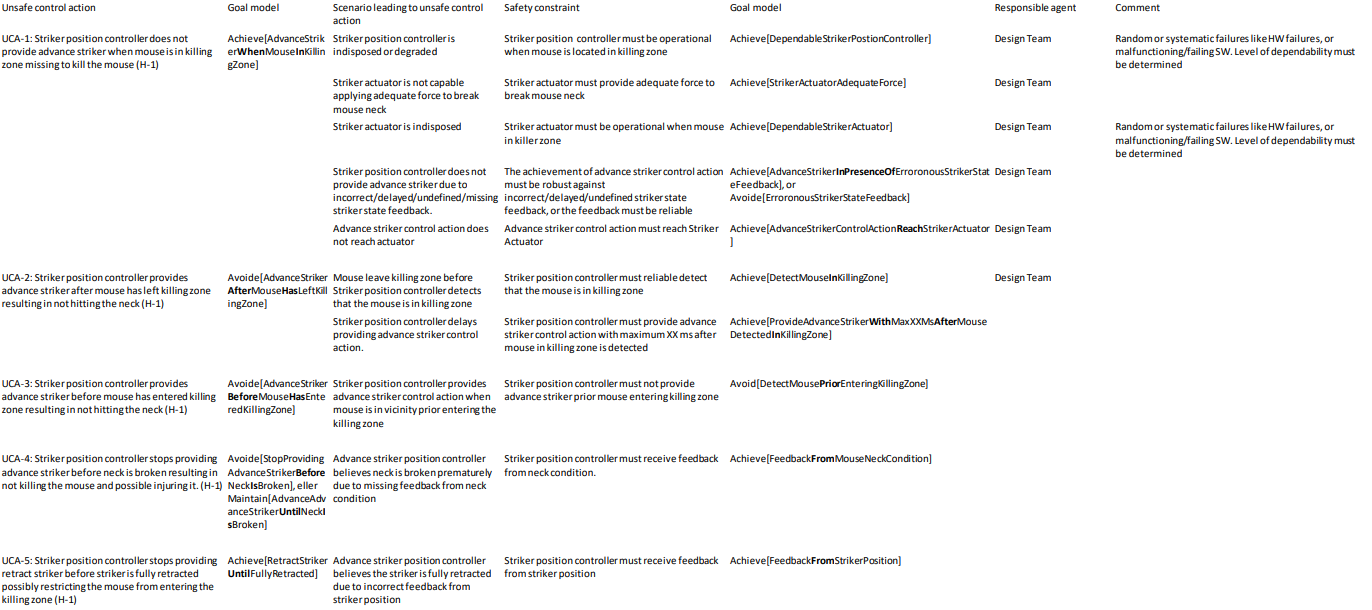
\includegraphics[width=\textwidth]{figures/STPÅ/step4_mus.PNG}\\
        \caption{Tapsscenarioer fra musefelle-eksempel.}
\end{figure}


\subsection{STPA sin rolle i CESM}

Det hierarkiske kontrolldiagrammet inneholder kontroller og den kontrollerte prosesse. Kontrolleren representerer aktøren i strukturen i CESM, dermed er det en aktørmodell. Men dette er bare utgangspunktet, og metoden adresserer de fleste av de andre modellene. En aksjon kan sies å være en funksjon som utføres av en aktør, dermed adressserer control action funksjonsmodellen (mekanismer i CESM). Videre skal man finne scenarioer for hvordan "Unsafe control actions" kan lede til fare definert i første steg gjennom såkalte guidewords. Deretter skal man undrsøke kontrollstrukturen for å finne scenarioer for hvordan sikkerhetsbegrensningene kan bli brutt. Dermed addresseres også målmodellen og modell for oppførsel av systemet, eller ev, hvordan man ikke vil at systemet skal oppføre seg. 

\begin{figure}[H]
    \centering
        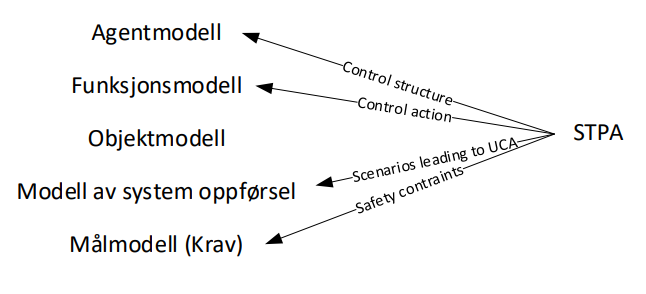
\includegraphics[width=0.7\textwidth]{figures/STPÅ/stpa_cesm.PNG}\\
        \caption{Hvordan de ullike delene av STPA relaterer til CESM-metamodellen.}
\end{figure}


\subsection{STPA vs FMECA}

STPA er konkurrerende med FMECA i å være en større og grundigere analyse av systemet. De leverer ofte liknende resultater. 

I STPA idenfiseres flere nyanser av feil. Dette fordi man, i analysen av UCA-ene, blir tvunget til å analysere funksjonene under spesifikke omstendigheter, eks "Providing causes hazard". Eksempel fra analyse av thrusterkontroller:

\begin{itemize}
    \item \textbf{Feilmoder FMECA}:
    \begin{itemize}
        \item Ingen pådragsreferanse
        \item Feil pådragsreferanse
    \end{itemize}
    \item \textbf{UCAs fra STPA}:
    \begin{itemize}
        \item Manglende pådragsreferanse
        \item Feil pådragsreferanse
        \item Sepunkt settes ved feil tidspunkt
        \item Setpunkt fjernes for fort
        \item Setpunkt holdes for lenge
    \end{itemize}
\end{itemize}

I tillegg er perspektivet på samhandling litt annerledes i de forskjellige metodene. I STPA er det "ovenfra og ned", og aktøren over prosessen har "ansvar" for prosessen, og man analyserer hvordan aktøren kan feile i sin kontroll. 


Vi ser også at i STPA har vi et predefinert sett med tap som UCAsene og hazardsene knyttes opp mot. I FMECA defineres effektene av feilene litt "on-the-go". SLik får man illustrert sammenhenger mellom aktører, funksjoner og konsekvenser i STPA, hvor dette ikke kommer like godt fram i FMECA.


\textbf{MERK}: FAST er ikke en konkurrerende analysemetode, men kan fungere som et godt supplement til begge metodene.
